\documentclass[11pt]{beamer}
\usetheme{Warsaw}
\usecolortheme {dolphin}
\definecolor{blueviolet}{HTML}{414A69}

\usepackage[utf8]{inputenc}
\usepackage{graphicx}

\usepackage[english,serbian]{babel}

\usepackage{amsmath}
\usepackage{amsfonts}
\usepackage{amssymb}
\usepackage{graphicx}
\usepackage{textcomp}
\usepackage{hyperref}

\author{Gorana Vučić, Vojkan Cvijović}
\title{Optimizacija kolonijom mrava za problem trgovačkog putnika}
%\setbeamercovered{transparent} 
%\setbeamertemplate{navigation symbols}{} 
%\logo{} 
\institute{Naučno izračunavanje\break  Matematički fakultet, Beograd} 
%\date{\today} 
%\subject{} 
\begin{document}

%1. slajd
\begin{frame}
\titlepage
\end{frame}

%2. slajd
\begin{frame}
\frametitle{Pregled}
\tableofcontents
\end{frame}

%3. slajd
\section{Uvod}
\subsection{Uopšteno}
\begin{frame}{}
  \begin{itemize}
  \item {\bf{ACO}} (eng.~{\em{ant colony optimization}})
    \begin{itemize}
    \item Algoritam zasnovan na ponašanju mrava i mravljih kolonija
    \item Pojam je uveo Marco Dorigo 1992. godine
    \item ACO pripada klasi algoritama inteligencije roja
    \end{itemize}
  \item {Primena algoritma je prikazana na rešavanju problema trgovačkog putnika}
  \item {Optimizacija kolonijom mrava predstavlja algoritam koji se koristi za nalaženje optimalnih putanja u potpuno povezanom grafu}

  \end{itemize}
\end{frame}

%4. slajd
\subsection{Ponašanje mrava}
\begin{frame}{}
    \begin{itemize}
    \item Ukoliko postavimo mrave u nepoznatu okolinu kako bi došli do izvora hrane u početku će se nasumično kretati
    \item Kada pronađu hranu pri povratku u koloniju ostavljaće trag feromona koji će privlačiti ostale mrave da se kreću u tom smeru
    \item Ostali mravi će početi da se kreću u smeru traga feromona, pojačavaće trag feromona i na taj način će privlačiti još mrava
    \item Nakon određenog vremena počinje da se odvija proces evaporacije odnosno isparavanje feromona, što je od velike koristi s obzirom da se pozicija hrane stalno menja
    \end{itemize}
\end{frame}


%5. slajd
\subsection{Ponašanje mrava u slučaju prepreke na putu}
\begin{frame}{}
      \begin{itemize}
      \item U početku verovatnoća da odaberu levi ili desni put je jednaka, polovina mrava će ići levim a druga polovina desnim putem
      \item Levi put je kraći $\implies$ ostaće jači trag feromona
      \item Kako vreme odmiče veći broj mrava će prolaziti tim putem, jačina feromona će biti veća i na kraju će se čitava kolonija kretati tim putem
        \begin{figure}
          \begin{flushright}
            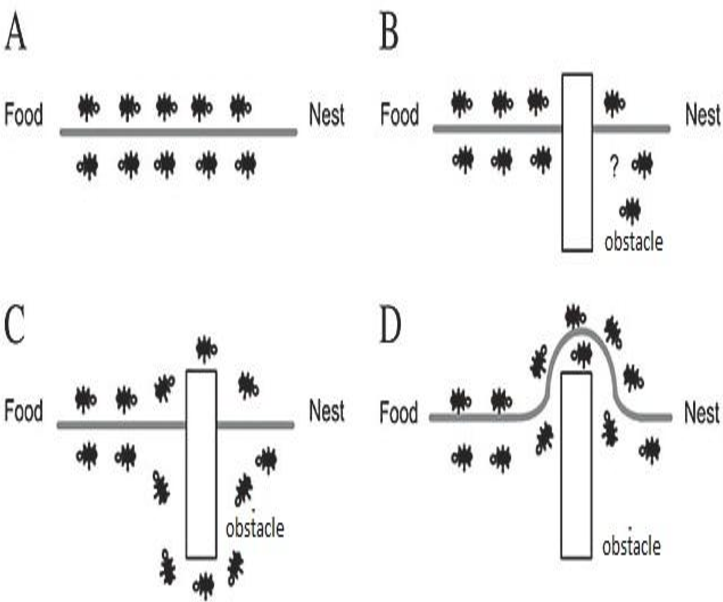
\includegraphics[scale=0.3]{../documentation/aco_obstacle.png}
          \end{flushright}
        \end{figure}
      \end{itemize}
\end{frame}


%% %6. slajd
%% \begin{frame}{}

%% \end{frame}


%7. slajd
\section{Primena ACO na TSP}
\begin{frame}{}
\frametitle{Problem trgovačkog putnika}
\begin{itemize}
  \item Jedan od najpozantijih problema iz grupe NP teških problema
  \item Trgovački putnik:
  	\begin{itemize}
  		\item Zna koje gradove treba da poseti
  		\item Zna udaljenost među gradovima
  		\item U obavezi je da svaki grad poseti tačno jednom i da se vrati u grad iz kog je pošao
  	\end{itemize}
  \item Rešenje se ogleda u tome da trgovački putnik odredi redosled gradova i da pritom putuje najoptimalnijom mogućom rutom
\end{itemize}
\end{frame}


%8. slajd
\subsection{ACO i parametri}
\begin{frame}{ACO algoritam za TSP i parametri}
\begin{itemize}
  		\item Algoritam se odvija u četiri koraka:
  		\begin{itemize} 
  		\item Na slučajan način odabere se $m$ od ukupno $n$ gradova ($m 	\leq n$) u koje se rasporedi po jedan mrav
  		\item Svaki mrav posećuje svaki grad tačno jedanput i u svakoj iteraciji ažurira listu gradova $J_{k}$ koje treba da poseti
  		\item Mrav $k$ koji se nalazi u gradu $i$ prelazi u grad $j$ gde je
  		$j \in J_{k}$ sa verovatnoćom:
  		\begin{equation}\label{1}
			p_{i,j}^k = {t_{i,j}^\alpha * distance_{i,j}^{-\beta} \over \sum_{l 			\in J_k}^{} t_{i,j}^\alpha * distance_{i,j}^{-\beta}}
		\end{equation}
		\item ...
  		\end{itemize} 
\end{itemize} 
\end{frame}


%9 slajd
\subsection{ACO algoritam}
\begin{frame}{ACO algoritam za TSP i parametri}
\begin{itemize}
  		\item Algoritam se odvija u četiri koraka:
  		\begin{itemize} 
		\item Neka je $L_{k}$ dužina puta $T_{k}$ koji je prešao mrav $k$ i $Q$ 		pogodno izabran pozitivan parametar. Neka važi: 

		\begin{figure}[h!]
		\begin{center}
			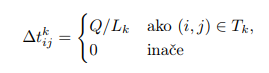
\includegraphics[scale=0.5]{formula.png}
		\end{center}
		\label{fig:formula}
		\end{figure}

		\begin{equation}\label{4}
		\Delta t_{i,j}  = \sum_{k=1}^{m} \Delta t^k_{i,j}
		\end{equation}
		Za pogodno izabran parametar $\rho \in$(0,1), feromonski tragovi se 			ažuriraju na osnovu formule  
		\begin{equation}\label{3}
			t_{i,j} = (1-\rho) * t_{i,j} + \Delta t_{i,j}
		\end{equation}
		
		Parametar $\rho$ predstavlja stepen isparavanja feromona, a $\Delta 			t_{i,j}$ pojačanje količine feromona na deonici ($i$,$j$).

  		

  		\end{itemize} 
\end{itemize} 
\end{frame}

\section{Implementacija}
\subsection{Klase}
\begin{frame}{}
\frametitle{Klase i metode koje su korišćene}
\begin{itemize}
  \item Korišćene su tri klase:
  	\begin{itemize}
  		\item $Graph$
  		\item $ACS$
  		\item $Ant$
  	\end{itemize}
  \item $Graph$ sadrži neke opšte informacije o gradovima kao što su:
  	\begin{itemize}
  		\item $distances$: predstavlja matricu rastojanja između gradova
  		\item $rank$: predstavlja broj gradova, važi da između svaka dva grada postoji put
  		\item $pheromone$: predstavlja matricu nivoa feromona između gradova
  	\end{itemize}
\end{itemize}
\end{frame}


\subsection{Klasa ACS i njene metode}
\begin{frame}{}
\frametitle{Klase i metode koje su korišćene}
\begin{itemize}
  \item $ACS$ - klasa koja se koristi za rešavanje problema putujućeg trgovca primenom ACO algoritma:
  	\begin{itemize}
  		\item $generations$: predstavlja broj iteracija samog algoritma
  		\item $ant\_count$: predstavlja broj mrava u svakoj iteraciji
  		\item $alpha$: parametar koji određuje uticaj feromona 
		\item $beta$: parametar koji određuje uticaj udaljenosti između gradova
		\item $rho$: parametar koji oređuje koja količina
starog feromona se prenosi u narednu iteraciju algoritma
		\item $Q$: pogodno izabran pozitivan parametar
  	\end{itemize}
  \item Klasa sadrži metode $update\_pheromone$ i $solve$.
\end{itemize}
\end{frame}

\subsection{Klasa Ant i njene metode}
\begin{frame}{}
\frametitle{Klase i metode koje su korišćene}
\begin{itemize}
  \item $Ant$ - klasa koja predstavlja jednog mrava u sistemu:
  	\begin{itemize}
  		\item $colony$: instanca klase ACS
  		\item $graph$: instanca grafa koji mrav obilazi
  		\item $total\_cost$: cena puta koju je mrav prešao 
		\item $visited\_nodes$: niz čvorova koje je mrav obišao
		\item $pheromone\_delta$: veličina feromona koju je mrav proizveo
		\item $unvisited\_nodes$: neposećeni čvorovi u grafu
		\item $start\_node$: početni čvor iz kog mrav polazi
		\item $visited\_nodes$: niz čvorova koje je mrav obišao
		\item $current\_node$: indeks čvora koji mrav trenutno obilazi
  	\end{itemize}
  \item Klasa sadrži metode $update\_pheromone\_delta$ i $select\_next\_node$.
\end{itemize}
\end{frame}


\section{Pokretanje i izgled rešenja}
\begin{frame}{}
\frametitle{Pokretanje i izgled rešenja}
\begin{itemize}
  \item Metodom $find\_optimal\_path$ se pokreće izvršavanje programa.
  \item Rešenje je dato u sledećem obliku:
  		\begin{figure}[h!]
		\begin{center}
			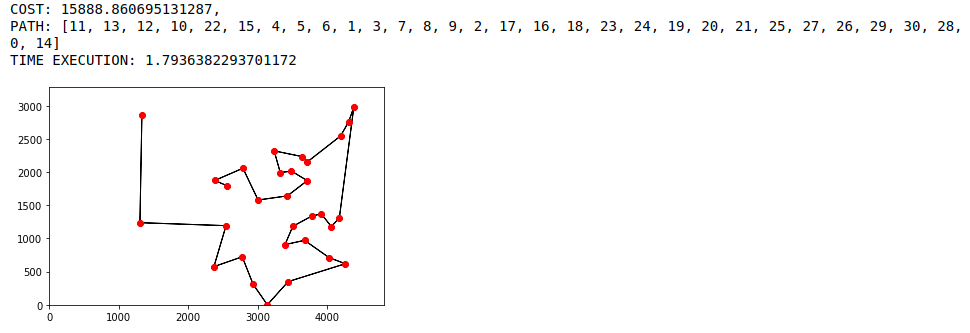
\includegraphics[scale=0.3]{opt.png}
		\end{center}
		\label{fig:optres}
		\end{figure}
\end{itemize}
\end{frame}


\section{Rezultati pokretanja}
\begin{frame}{}
\frametitle{Rezultati pokretanja}
\begin{itemize}
  \item Najbolje rešenje je dobijeno za sledeće parametre:
	\begin{itemize}
		\item $ant\_count = 10$
		\item $generations = 100$
		\item $alpha = 1.0$
		\item $beta = 10.0$
		\item $rho = 0.5$
		\item $q = 10$

	\end{itemize}
	\item Prosečno vreme izvršavanja za zadate parametre je 5.32s, najbolje rešenje iznosi 7663.58 sa vremenom izvršavanja 5.56s.

\end{itemize}
\end{frame}

\subsection{Promena $\alpha$}
\begin{frame}{}
\frametitle{Promena $\alpha$}
\begin{itemize}
  \item Najbolje rešenje je dobijeno za $alpha = 1$:
	 \begin{figure}[h!]
		\begin{center}
			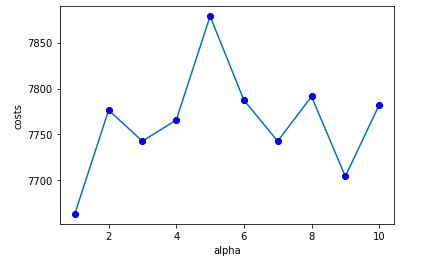
\includegraphics[scale=0.3]{alpha.png}
		\end{center}
		\label{fig:optres}
	\end{figure}

\end{itemize}
\end{frame}

\subsection{Promena $\beta$}
\begin{frame}{}
\frametitle{Promena $\beta$}
\begin{itemize}
  \item Najbolje rešenje je dobijeno za $beta = 9$:
	 \begin{figure}[h!]
		\begin{center}
			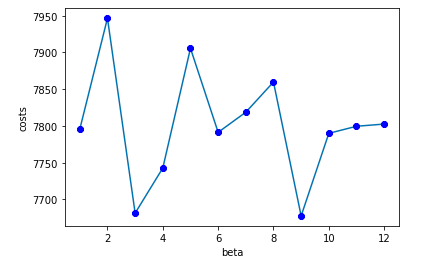
\includegraphics[scale=0.3]{beta.png}
		\end{center}
		\label{fig:optres}
	\end{figure}

\end{itemize}
\end{frame}

\subsection{Promena $\rho$}
\begin{frame}{}
\frametitle{Promena $\rho$}
\begin{itemize}
  \item Najbolje rešenje je dobijeno za $rho = 1.0$:
	 \begin{figure}[h!]
		\begin{center}
			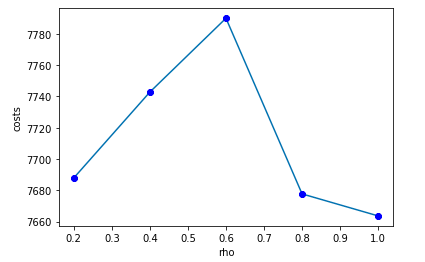
\includegraphics[scale=0.3]{rho.png}
		\end{center}
		\label{fig:optres}
	\end{figure}

\end{itemize}
\end{frame}

\begin{frame}{Literatura}
  \frametitle{Literatura}
  {\small
    \begin{itemize}
    \item Stefan Mišković. Optimizacija kolonijom mrava. \url{http://poincare.
matf.bg.ac.rs/~stefan/ri/aco.pdf}.
    \item Dorian Gaertner and Keith Clark. On optimal parameters for ant
colony optimization algorithms. In Proceedings of the International
Conference on Artificial Intelligence 2005, pages 83–89. CSREA Press,
2005.
    \item Ivan Brezina Jr. and Zuzana Čičková. In Solving the Travelling Sale-
sman Problem Using the Ant Colony Optimization, 2011.
    \item K. M. Shweta and A. Singh. In An effect and analysis of parameter on
ant colony optimization for solving travelling salesman problem, page
222–229. IJCSMC, 2013.
	\item Matplotlib library. on-line at: \url{https://matplotlib.org/}.
    \end{itemize}
  }
\end{frame}

\begin{frame}{}
  \center{\huge Hvala na pažnji!}
\end{frame}


\end{document}
